%==============================================================================
% ETHASL - Template for student projects at the ASL
% 2013.10: Péter Fankhauser
% This template is based on the IMRT Latex template by Eric A. Mueller.
%==============================================================================

\documentclass[10pt,twoside,a4paper]{report}

\usepackage{pdfpages}

% ETHASL package
% TODO Choose options according to your project
% som/bt/st/mt: Studies on Mechatronics, Bachelor Thesis, Semester Thesis, Master Thesis
% fs/hs: Spring term, Autumn term
% german/english: German/English
\usepackage[bt,hs,english]{packages/ethasl}

% Graphics
\usepackage{graphicx}
\graphicspath{ {./images/} }

% Nomenclature
\usepackage{nomencl}
\makenomenclature

% Smart reference
\usepackage[]{hyperref}
% colorlinks=true, allcolors=blue

% Other
\usepackage{etoolbox} % For using ifstrequal function for nomenclature grouping 
% \usepackage{subfig} % For grouping figures together in a single row

%%%%%%%%%%%%%%%%%%%%%%%%%%%%%%%%%%%%%%%%%%%%%%%%%%%%%%%%%%%%%%%%%%%%%%%%%%%%%%%
% LaTeX preamble
%%%%%%%%%%%%%%%%%%%%%%%%%%%%%%%%%%%%%%%%%%%%%%%%%%%%%%%%%%%%%%%%%%%%%%%%%%%%%%%
% Encoding settings
\usepackage[utf8]{inputenc}
\usepackage[OT1]{fontenc}

% Paper size
\usepackage{a4}

% Headings
\usepackage{fancyhdr}

% More symbols
\usepackage{textcomp}\usepackage{gensymb}

% Math support for Times font
%\usepackage{txfonts}

% ISO date
\usepackage[english]{isodate}

% Multi column
\usepackage{multicol}

% Figures
\usepackage{graphicx}

% Subfigures (obsolete)
\usepackage{subfigure}

% Bibliography
\usepackage[numbers]{natbib}

% Nicer tables
\usepackage{booktabs}
\usepackage{array}
\usepackage{multirow}

% Colors
\usepackage{color}
\usepackage{colortbl}
\definecolor{black}{rgb}{0,0,0}
\definecolor{white}{rgb}{1,1,1}
\definecolor{darkred}{rgb}{0.5,0,0}
\definecolor{darkgreen}{rgb}{0,0.5,0}
\definecolor{darkblue}{rgb}{0,0,0.5}

% Additional math functionality
\usepackage{amsmath}
\usepackage{amssymb}

% Nice fractions
\usepackage{nicefrac}

% Upper case greek letters
\usepackage{upgreek}

% ISO math notation
\usepackage{isomath}
\renewcommand{\vec}{\vectorsym}
\newcommand{\mat}{\matrixsym}

% Units
\usepackage{units}

% Rotated objects
\usepackage{rotating}

% Indent
\setlength{\parindent}{0em}

% Include PDF pages
\usepackage{pdfpages}
\includepdfset{pages={-}, frame=true, pagecommand={\thispagestyle{fancy}}}

% Headings
\rhead[\thepage]{\nouppercase{\rightmark}}
\lhead[\nouppercase{\leftmark}]{\thepage}
\cfoot{}

% Gantt chart
\usepackage{pgfgantt}

% Links (last package)
\PassOptionsToPackage{hyphens}{url}\usepackage{hyperref}

% Clever references (has to be loaded after hyperref)
\usepackage{cleveref}


%%%%%%%%%%%%%%%%%%%%%%%%%%%%%%%%%%%%%%%%%%%%%%%%%%%%%%%%%%%%%%%%%%%%%%%%%%%%%%%
% Title page
%%%%%%%%%%%%%%%%%%%%%%%%%%%%%%%%%%%%%%%%%%%%%%%%%%%%%%%%%%%%%%%%%%%%%%%%%%%%%%%
\begin{document}

\title{Unified Path Following for Hybrid VTOLs}

\studentA{Junwoo Hwang}

\supervisionA{Jaeyoung Lim / Florian Achermann}
\supervisionB{David Rohr / Thomas Stastny}
\supervisionC{Roland Siegwart / Hwangnam Kim}

% TODO: How to add professors & TJ?

\projectYear{\the\year} % This year

\maketitle
\pagestyle{plain}
\pagenumbering{roman}

%%%%%%%%%%%%%%%%%%%%%%%%%%%%%%%%%%%%%%%%%%%%%%%%%%%%%%%%%%%%%%%%%%%%%%%%%%%%%%%
% Declaration of originality
%%%%%%%%%%%%%%%%%%%%%%%%%%%%%%%%%%%%%%%%%%%%%%%%%%%%%%%%%%%%%%%%%%%%%%%%%%%%%%%
% \pagestyle{empty}
% TODO Modify placeholders in declaration.tex
%% TODO Add title, student first/last name, supervisor first/last name.

\section*{Declaration of Originality}

\vspace{1cm}

I hereby declare that the written work I have submitted entitled

\vspace{0.5cm}

% TODO Add title
\textbf{Your Project Title}

\vspace{0.5cm}

is original work which I alone have authored and which is written in my own words.\footnote{Co-authored work: The signatures of all authors are required. Each signature attests to the originality of the entire piece of written work in its final form.}

\vspace{1cm}

\textbf{Author(s)}

\vspace{0.5cm}

\begin{tabular}{ p{5cm} p{5cm} }
% TODO Add student first/last name
  First name & Last name \\
\end{tabular}

\vspace{0.5cm}

\textbf{Student supervisor(s)}

\vspace{0.5cm}

\begin{tabular}{ p{5cm} p{5cm} }
% TODO Add supervisor first/last name
  First name & Last name \\
\end{tabular}

\vspace{0.5cm}

\textbf{Supervising lecturer}

\vspace{0.5cm}

\begin{tabular}{ p{5cm} p{5cm} }
  Roland & Siegwart \\
\end{tabular}

\vspace{1cm}

With the signature I declare that I have been informed regarding normal academic citation rules and that I have read and understood the information on 'Citation etiquette' (\url{https://www.ethz.ch/content/dam/ethz/main/education/rechtliches-abschluesse/leistungskontrollen/plagiarism-citationetiquette.pdf}).
The citation conventions usual to the discipline in question here have been respected.

\vspace{0.5cm}

The above written work may be tested electronically for plagiarism.

\vspace{4cm}

\begin{tabular}{ p{5cm} p{1cm} p{5cm} }
  \cline{1-1} \cline{3-3}
  Place and date & & Signature \\
\end{tabular}


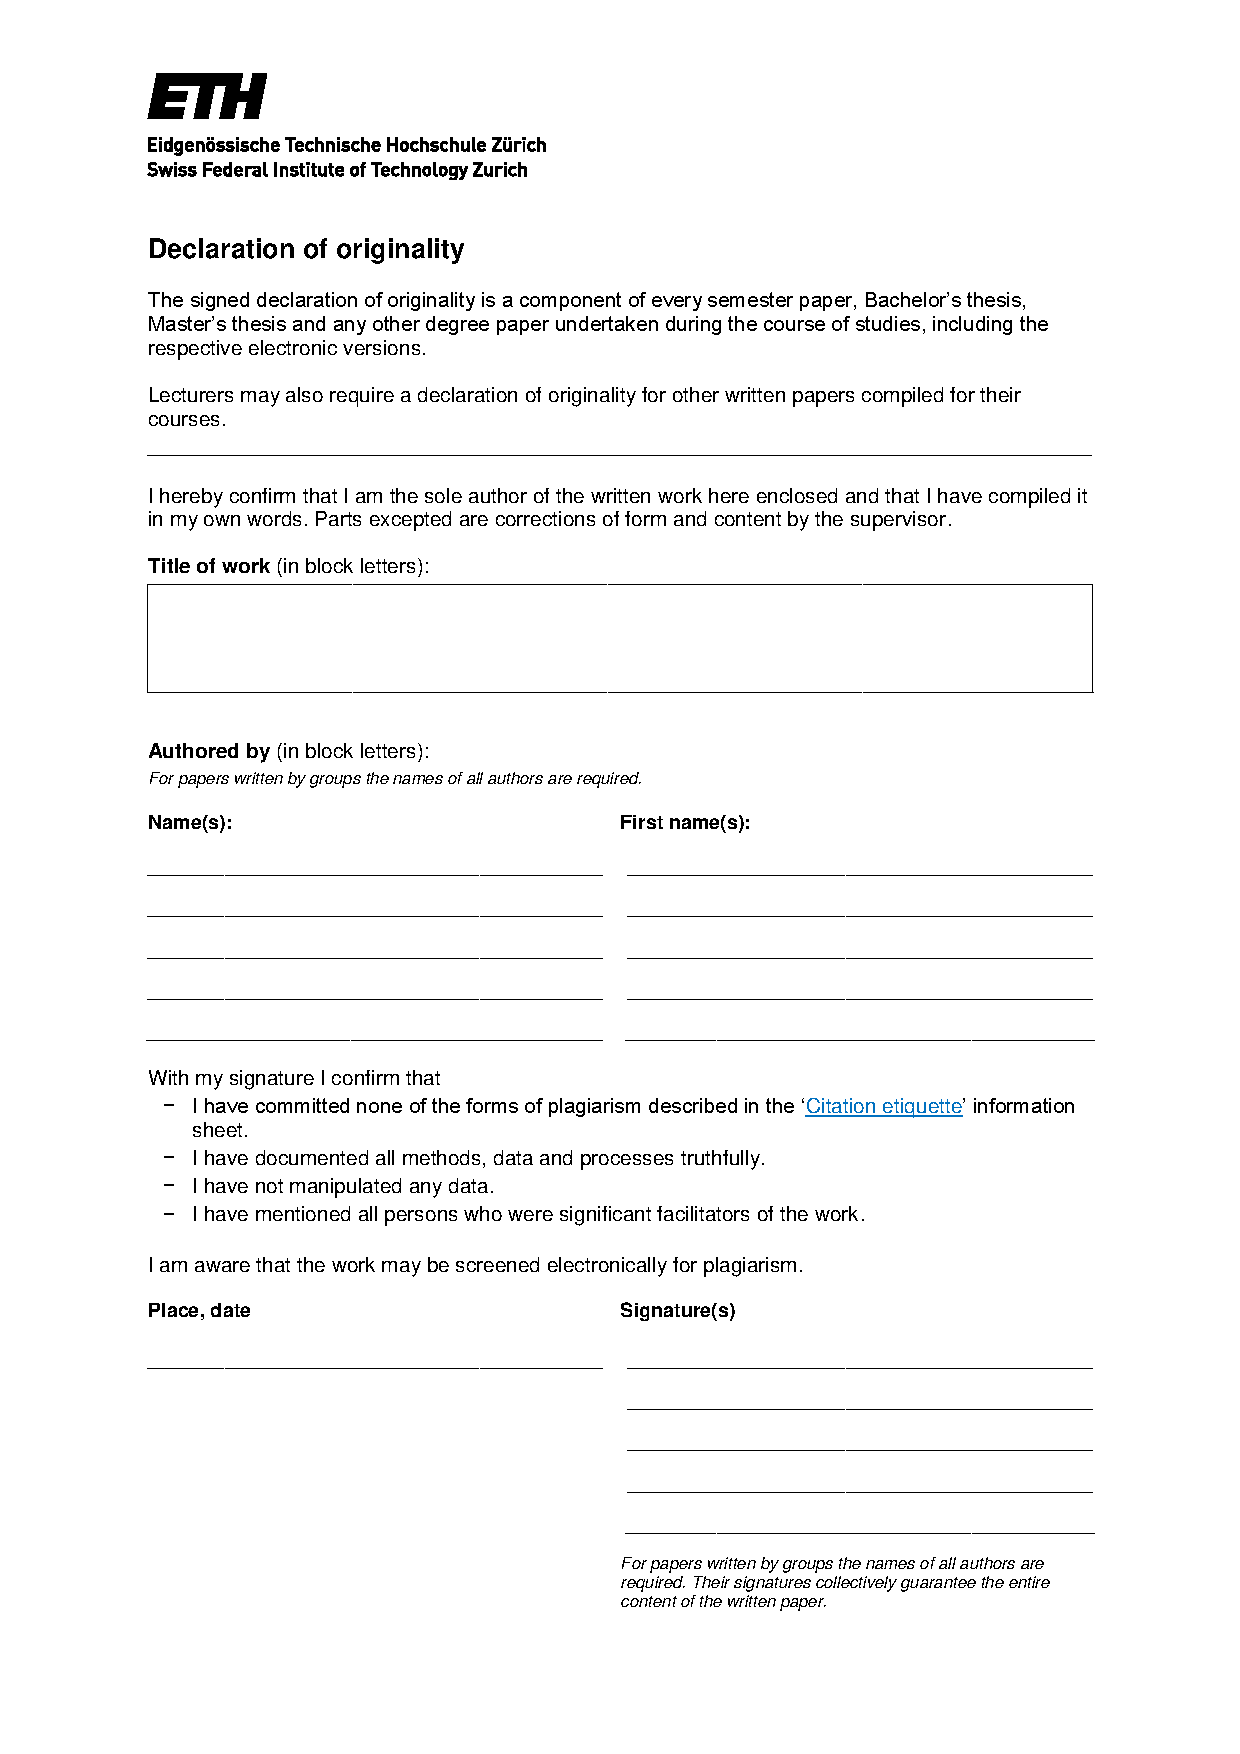
\includepdf[pagecommand={}]{chapters/declaration-originality.pdf}

%%%%%%%%%%%%%%%%%%%%%%%%%%%%%%%%%%%%%%%%%%%%%%%%%%%%%%%%%%%%%%%%%%%%%%%%%%%%%%%
% Table on contents
%%%%%%%%%%%%%%%%%%%%%%%%%%%%%%%%%%%%%%%%%%%%%%%%%%%%%%%%%%%%%%%%%%%%%%%%%%%%%%%
% Table of Contents depth (TODO change if necessary)
\setcounter{tocdepth}{2}

\renewcommand*\contentsname{Table of Contents}
\tableofcontents
% \cleardoublepage

%%%%%%%%%%%%%%%%%%%%%%%%%%%%%%%%%%%%%%%%%%%%%%%%%%%%%%%%%%%%%%%%%%%%%%%%%%%%%%%
% Main content
%%%%%%%%%%%%%%%%%%%%%%%%%%%%%%%%%%%%%%%%%%%%%%%%%%%%%%%%%%%%%%%%%%%%%%%%%%%%%%%
\chapter*{Abstract}
\addcontentsline{toc}{chapter}{Abstract}

With the advancement of low-cost electronics and UAV components, an interesting hybrid vehicle type so-called 'Hybrid VTOL' has been under the spotlight of academia and researchers' interest recently. Due to its versatility of utilizing both modes of operation from two distinct vehicle regimes: Multirotor and Fixed Wing, this breed of vehicle can fly further in an energy-efficient manner, meanwhile preserving the capability to launch and land in a small confined space when needed.

However, Hybrid VTOLs usually have a decoupled Path Following a control strategy depending on its mode of operation. Although this approach works in a practical sense, both of the control strategies fail to capture the overall flexibility of the system.

In this thesis, a new Vector Field based Path Following formulation is derived and shown for supporting both fixed-wing and multirotor modes of operation.

\chapter*{Acknowledgements}
\addcontentsline{toc}{chapter}{Acknowledgements} %Not 100% certain why this is ncessary but anyways

I would like to express my upmost gratitude for everyone who helped me throughout the journey of making this Bachelor Thesis project possible. As Thomas wrote in his PhD dissertation\cite{stastny_low-altitude_2020}, ASL is truly like nowhere else, and has been, and will be a big part of my source of motivation in Robotics.\\

When I came across ASL's AtlantikSolar project in 2016 during my first year in Highschool, I was truly fascinated by the dedication and expertise ASL had to make such an incredible project possible. And undoubtedly, that led me to the field of Robotics, so having done this 4 Months long research at the foundation where my whole journey started was a mesmerizing experience. I will be missing the Coffee Kiosk at ASL, and hope to return in the near future!\\

Also, thank you Auterion for an incredible internship opportunity, and for helping me throughout the duration of the project!

% \chapter*{Preface}
\addcontentsline{toc}{chapter}{Preface}

This thesis was written because ...
% \cleardoublepage

% Set title used in nomenclature library
\renewcommand{\nomname}{Symbols}

%% This code creates the groups
% -----------------------------------------
\renewcommand\nomgroup[1]{%
  \item[\bfseries
  \ifstrequal{#1}{V}{Vehicle constraints}{%
  \ifstrequal{#1}{P}{Path Following parameters}{%
  \ifstrequal{#1}{S}{Vehicle states}{}}}%
]}
% -----------------------------------------

\nomenclature[V]{$V_{min}$}{Minimum Speed Vehicle can achieve}
\nomenclature[V]{$V_{nom}$}{Nominal Speed Vehicle can achieve (cruise speed for Fixed Wing)}
\nomenclature[V]{$V_{max}$}{Maximum Speed vehicle can achieve}
\nomenclature[P]{$V_{path}$}{Desired speed on path}
\nomenclature[P]{$V_{approach}$}{Desired approaching speed orthogonal to the path}
\nomenclature[P]{$V_{ref}^{\parallel}$}{Target velocity component parallel to path}
\nomenclature[P]{$V_{ref}^{\perp}$}{Target velocity component orthogonal (towards) to path}
\nomenclature[P]{$e$}{Cross track error distance to the path}
\nomenclature[P]{$e_{b}$}{Track error boundary}
\nomenclature[P]{$t_{const}$}{Track error boundary time constant}
\nomenclature[P]{$\hat{t_p}$}{Unit tangent vector of the path segment}
\nomenclature[P]{$\overline{e}$}{Normalized track error}
\nomenclature[S]{$\lambda$}{Course over ground}
\nomenclature[S]{$\xi$}{Heading}

% Make nomenclature chapter
\printnomenclature
\label{sec:symbols}
\addcontentsline{toc}{chapter}{Symbols}

% Indices
\section*{Indices}
\begin{tabbing}
 \hspace*{1.6cm}  \= \kill
 $x$ \> x axis \\[0.5ex]
 $y$ \> y axis \\[0.5ex]
\end{tabbing}

% Acronyms
\section*{Acronyms and Abbreviations}
\begin{tabbing}
 \hspace*{1.6cm}  \= \kill
 ETH \> Eidgenössische Technische Hochschule \\[0.5ex]
 UAV \> Unmanned Aerial Vehicle \\[0.5ex]
\end{tabbing}
% \cleardoublepage

%%%%%%%%%%%%%%%%%%%%%%%%%%%%%%%%%%%%%%%%%%%%%%%%%%%%%%%%%%%%%%%%%%%%%%%%%%%%%%%
% Chapters custom
%%%%%%%%%%%%%%%%%%%%%%%%%%%%%%%%%%%%%%%%%%%%%%%%%%%%%%%%%%%%%%%%%%%%%%%%%%%%%%%
\pagestyle{fancy}
\pagenumbering{arabic}

\chapter{Introduction}
\label{sec:introduction}

\section{Motivation}
Hybrid VTOLs are particularly interesting vehicle to study, which has an intermediate mode as either a Multirotor, or a Fixed Wing.

\begin{figure}[h]
\centering
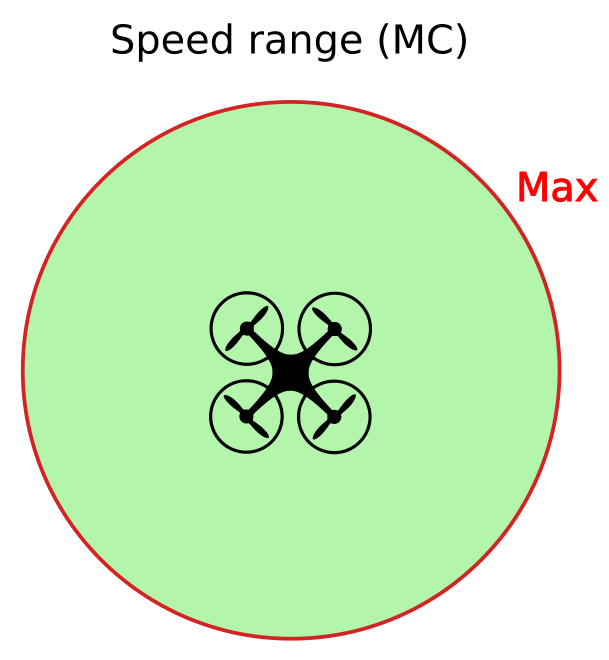
\includegraphics[width=0.3\textwidth]{MC_Velocity_Range}
\caption{Multirotor velocity range}
\end{figure}

\begin{figure}[h]
\centering
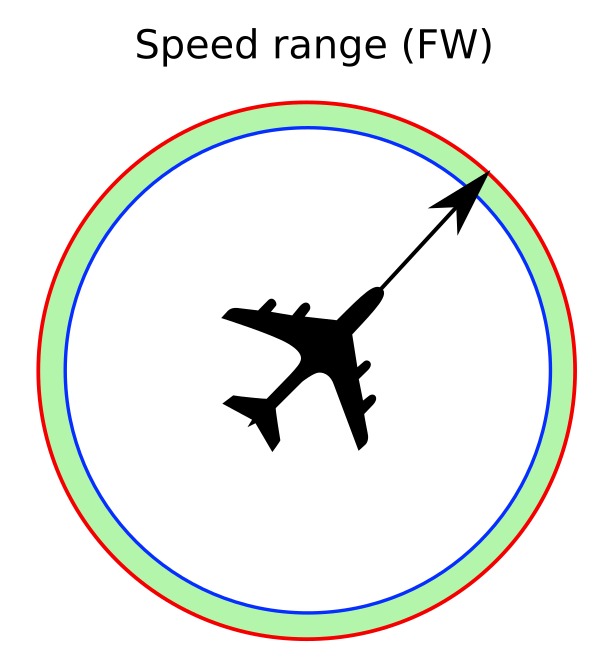
\includegraphics[width=0.3\textwidth]{FW_Velocity_Range}
\caption{Fixed Wing velocity range}
\end{figure}

\section{Goal of this Project}
The goal of this thesis is to construct a unified path following guidance that can be utilized both by Multirotor and Fixed Wing vehicles, thereby also allowing the usage on Hybrid VTOL vehicles.

\section{Contributions}
This thesis, to our best knowledge, describes the first unified path following guidance that specifically accounts for the maneuverability envelope of a Hybrid VTOL.

\section{Overview}
This thesis is structured as following:

\begin{enumerate}
    \item In Problem Definition, we examine the path following problem in detail, and come up with the terminologies as well as the constraints that needs to be respected
    \item In Methods, we present 3 different formulations including the base method (from a past publication) and discuss the differences between them
    \item In Evaluation, we evaluate the formulations against the constraints and desired characteristics defined before
    \item In Conclusion, we determine which formulation is the best, and the use cases based on the evaluation
\end{enumerate}
% \cleardoublepage

\chapter{Related Work}
\label{ch:related_work}

\section{Path Following Methods}
\label{sec:path_following_methods}

There are different methods in the field of path-following control. Such as Vector field, Virtual target pursuit, Nonlinear, Feedback linearization, Optimal control, Model predictive control to name a few.

\subsection{Vector Field Method}
\label{subsec:vector_field_method}

\begin{figure}[h] % Fix position in document via 'h'
    \centering
    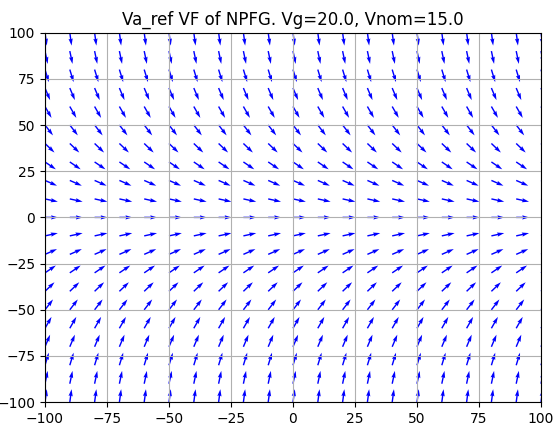
\includegraphics[width=0.7\textwidth]{vector_field_method_example}
    \caption{Visual representation of a Vector Field. Path is at Y=0 with the direction of +X}
\label{fig:vf_example}
\end{figure}

Vector Field method is based on generating a field of vectors around the path that when the vehicle follows the directions defined by the vectors, it will converge to the path\cite{stastny_flying_2019}\cite{sharma_vector_nodate}.\\

Since the Vector Field approach is simple (geometry), and easily extendable (vector field can be interpreted by both multirotor and fixed wing), it was chosen as the basis for the formulation in this thesis.

\subsection{Virtual Target Pursuit Method}
One of the most intuitive way to achieve path following is to have a virtual target point on the path that the vehicle chases. Also known as 'carrot chasing' method (imagine placing a carrot, and a horse blindly follows it. If you can steer the carrot cleverly, you can have an accurately path-following horse!), this method includes for example widely used L1 guidance law\cite{park_new_2004}, especially for fixed wing and multirotor applications in open-source autopilot software.

\section{Path Following on Hybrid VTOL}
Although almost no research on using a unified path following guidance for a Hybrid VTOL was conducted in the past, one study\cite{zhou_incremental_nodate} showed an 'Incremental nonlinear dynamic inversion' based path following for both multirotor and fixed-wing modes operation of a hybrid quad-plane. This study utilized the same concept as this thesis of the Vector Field method to generate desired ground velocity vector.\\

However, it assumed an arbitrary constant speed of 2.0 m/s for a multirotor, which severely under-utilizes the wide speed range of a multirotor. Also, having a constant speed means the ground track of converging to the path will always form arcs, which is also not how an operator would assume the vehicle to move and is severely under-utilizing the omnidirectional acceleration capability of a multirotor.
% \cleardoublepage

\chapter{Problem Definition}
\label{ch:problem_definition}

The path-following problem is to generate a desired command to guide a vehicle at a given initial configuration (position, velocity, and heading) onto a path, then have it move towards the desired direction. Unlike a conventional multirotor or a fixed wing, Hybrid VTOL can utilize both modes of the vehicle.\\

We must come up with a vector field of desired ground velocities ($V_{ref}$) on a 2D plane (vertical control isn't considered). The sections below define the set of requirements that an ideal Path Following guidance for Hybrid VTOL should incorporate.

\section{Output of the Path Following Guidance}
The output of a vector field based path following guidance is a desired velocity vector. And the low-level controller is expected to actuate the vehicle to achieve the desired velocity profile.

In some papers additional outputs like lateral acceleration, heading angle, etc are also formulated. However to simplify the application we do not constrain the guidance algorithm to also include any of those outputs.

\section{Approaching \& On-path Velocity Constraints}
\label{seq:approach_on_path_vel_constraints}

To abide by the user-specified path following behavior, which is $V_{path}$ for the desired speed on the path, and $V_{approach}$ for desired approaching speed orthogonal to the path outside the track error boundary($e_b$), the following conditions must be satisfied:

\begin{equation}
    V_{ref}^{\perp}(e)=\begin{cases}
    V_{approach}& \text{$e > e_b$}\\
    0& \text{if $e = 0$}
\end{cases}
\label{eq:v_orth_constraints}
\end{equation}

\begin{equation}
    V_{ref}^{\parallel}(e)=\begin{cases}
    0& \text{if $e > e_b$}\\
    V_{path}& \text{if $e = 0$}
\end{cases}
\label{eq:v_parallel_constraints}
\end{equation}

\section{Multirotor Behavior Constraints}

Since the multirotor mode of operation is capable of coming to a complete stop ($V_{ref} = 0$), and has an acceleration control in any desired direction irrelevant to the heading, we can define the following constraints:

\begin{equation}
\begin{split}
    ||V_{ref}|| < V_{max}\\
    ||\frac{d}{dt}V_{ref}|| < a_{max}^{mc}
\end{split}
\label{eq:multirotor_problem_definition}
\end{equation}

\section{Fixedwing Behavior Constraints}
Since the fixed wing mode of operation has essentially almost no control over the forward velocity ($V_{ref} = V_{nom}$), and only has a lateral acceleration control using roll angle manipulation, we can define the following constraints:

\begin{equation}
\begin{split}
    ||V_{ref}|| = V_{nom}\\
    ||a_{N}|| < a_{l, max}^{fw}
\end{split}
\label{eq:fixedwing_problem_definition}
\end{equation}

\section{Monotonicity Objective}
Ideally, the magnitude of the desired ground velocity vector field should be monotonic, meaning while approaching the path, the norm of the desired velocity vector should not increase and decrease at any two points in time.\\

Practically speaking, this ensures a smooth (vehicle either only brakes or accelerates) path approaching behavior and intuitively would prevent excessive use of acceleration. Therefore, the velocity vector field should satisfy only one of the conditions below.

\begin{equation}
    \frac{d}{dt}||V_{ref}(e)||=\begin{cases}
    \geq 0& \text{Monotonically increasing}\\
    \leq 0& \text{Monotonically decreasing}
\end{cases}
\end{equation}

\section{Convergence Time Objective}
Realistically, the path-following algorithm can't track a path with an absolute track error of zero. However, borrowing the concept of 'settling time' from control theory, we can classify the vehicle as converged to the path if the track error is within a certain threshold.\\

Therefore, the idealistic path following guidance should minimize the time of reaching track error of $e_{end}$, starting from a fixed starting track error $e_{start}$ (these values must be fixed to a sane value, such as $e_{end}$ as 5\% of $e_{start}$, and $e_{start}$ as the biggest track error boundary out of all algorithms in comparison).\\

And since we decouple a path parallel/orthogonal components of the desired ground velocity vector field, convergence time can be formulated like following.

\begin{equation}
\begin{split}
T_{conv} &= \int^{e_{end}}_{e_{start}}dt\\
&= -\int^{e_{end}}_{e_{start}}\frac{1}{V_{ref}^{\perp}(e)}de
\end{split}
\label{eq:convergence_time_definition}
\end{equation}
% \cleardoublepage

% Methods
\chapter{Methods}
\label{ch:methods}

\section{Constant Velocity Path Following (Unicyclic)}

As a base method to improve on, a Nonlinear Path Following Guidance\cite{stastny_flying_2019} for a Fixed Wing vehicle was chosen because the Fixed Wing presents the most conservative and constrained platform, and thus can be extended easily to incorporate a more agile platform (e.g. Multirotor).\\

Since Fixed Wing has a relatively constant forward speed, the algorithm thus assumes a 'unicyclic' motion, as if the vehicle was a person riding a unicycle with a constant speed. This means that only the direction of travel may change (heading), and not its speed.

\begin{figure}[h]
\centering
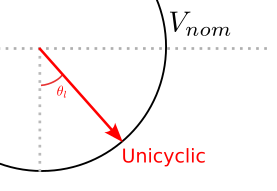
\includegraphics[width=0.7\textwidth]{Unicyclic_Formulation}
\caption{Unicyclic Formulation}
\label{fig:unicyclic_formulation}
\end{figure}

Here first the track error boundary gets defined proportional to the nominal speed $V_{nom}$. This is to make the path following magnitude independent and thus have a fixed convergence time. And the time constant $\tau_{const}$ can be set by the user, which in turn will define the acceleration that occurs when following the vector field.

\begin{equation}
    e_b = V_{nom} \cdot \tau_{const}
\label{eq:unicyclic_track_error_boundary}
\end{equation}

Here the look ahead angle $\theta_l$ is defined by the normalized track error $\overline{e}$, as in \cite{stastny_low-altitude_2020} defined in \autoref{eq:unicyclic_quadratic_laa_curve}.

\begin{equation}
    \theta_l = \frac{\pi}{2}(1-\overline{e})^2
\label{eq:unicyclic_quadratic_laa_curve}
\end{equation}

As shown in \autoref{fig:unicyclic_formulation}, when a desired course angle ($\theta_l$, relative to $\hat{t_p}$) is given, the desired ground velocity in the absence of wind essentially becomes $V_ref(e) = V_{nom} \cdot \hat{l}(e)$, where $\hat{l}$ is the unit vector pointing in the direction of a desired course angle.\\

This leads to the final reference velocity calculation like following

\begin{equation}
    \begin{split}
        V_{ref}^{\perp} &= V_{nom} \cdot cos(\theta_l)\\
        V_{ref}^{\parallel} &= V_{nom} \cdot sin(\theta_l)
    \end{split}
\label{eq:hybrid_velocity_components}
\end{equation}

Then (in the original formulation $V_{nom}$ is ignored in the absence of wind, and only heading error gets calculated) the heading error proportionally commands a lateral acceleration, which brings the vehicle on its desired heading, achieving the desired course angle.\\

Therefore the estimation of the vehicle's heading is a crucial factor in this formulation, which is why it isn't ideal for multirotor use cases since it doesn't have an acceleration capability tied to the heading.

\section{Variable Velocity Path Following (Hybrid)}

To overcome the aforementioned limitation of the Unicyclic formulation, a new 'Hybrid' formulation is presented. It is essentially an adaptation of the Unicyclic formulation to account for a flexible velocity range  of a Multirotor and a different meaning behind the vector field itself.

\begin{figure}[h]
\centering
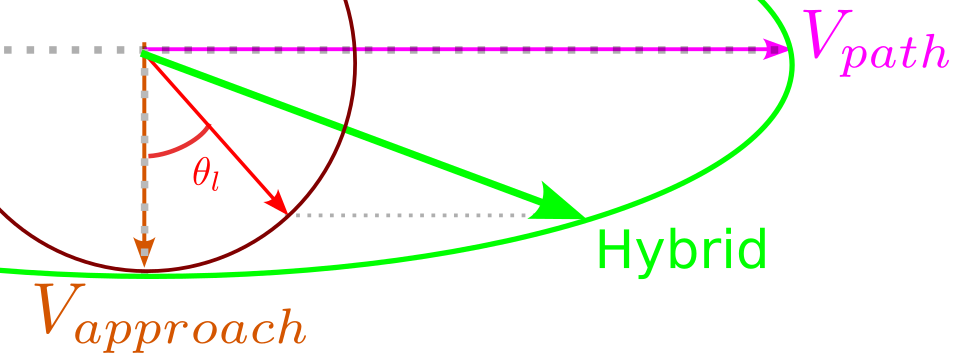
\includegraphics[width=0.7\textwidth]{Hybrid_Formulation}
\caption{Hybrid Formulation}
\end{figure}

Unlike the unicyclic method, hybrid has a variable $V_{path}$ component parallel to path, and $V_{approach}$ component orthogonal to path. And it is essentially an ellipse that is stretched in each axis to match the approach \& on-path constraints described in \autoref{seq:approach_on_path_vel_constraints}.

Track error boundary gets defined very similarly to the Unicyclic case, proportional to the approach speed $V_{approach}$. This was done because the convergence time depends on the orthogonal velocity curve. And the time constant $\tau_{const}$ can be set by the user, which in turn will define the acceleration that occurs when following the vector field.

\begin{equation}
    e_b = V_{approach} \cdot \tau_{const}
\label{eq:hybrid_track_error_boundary}
\end{equation}

Here the look ahead angle $\theta_l$ is defined by the normalized track error $\overline{e}$, as in \cite{stastny_low-altitude_2020} defined in \autoref{eq:hybrid_quadratic_laa_curve}.

\begin{equation}
    \theta_l = \frac{\pi}{2}(1-\overline{e})^2
\label{eq:hybrid_quadratic_laa_curve}
\end{equation}

This leads to the final reference velocity calculation like following

\begin{equation}
    \begin{split}
        V_{ref}^{\perp} &= V_{approach} \cdot cos(\theta_l)\\
        V_{ref}^{\parallel} &= V_{path} \cdot sin(\theta_l)
    \end{split}
\label{eq:hybrid_velocity_components}
\end{equation}

Along with it, the interpretation of the Velocity vector field is not just in terms of the desired course angle, but actually incorporates the exact velocity vector vehicle would need to achieve as shown in \autoref{fig:mc_fw_vector_field_pipeline}.

\begin{figure}[h]
\centering
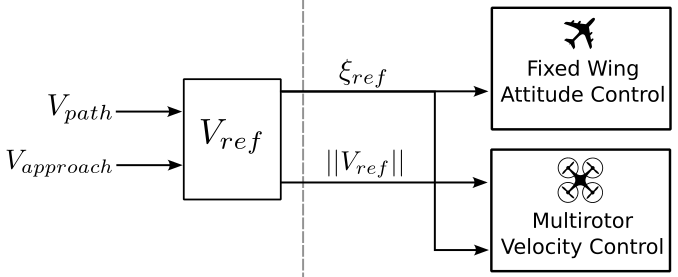
\includegraphics[width=0.7\textwidth]{VF_MC_FW_Pipeline}
\caption{Multirotor and Fixedwing control pipeline from the Vector Field}
\label{fig:mc_fw_vector_field_pipeline}
\end{figure}

This is possible because a multirotor can follow any velocity setpoint in any condition/heading. Furthermore, it doesn't get affected as much as in fixed wing case, so we can assume that any sane velocity setpoint within the vehicle's capability is feasible.\\

Notice how only the desired heading $\xi_{ref}$ is taken for fixed wing attitude control, and for multirotor the full velocity vector $V_{ref}$ is taken as an input.
% \cleardoublepage

% Evaluation
\chapter{Evaluation}
\label{sec:evaluation}

\section{Approach \& On-path Velocity Constraint}

As expected, the $V_{approach}$ and $V_{path}$ is only expected in the Hybrid formulation.

\subsection{Low Speed On Path}

\includegraphics[width=0.7\textwidth]{VPath_0}

For a case where we desire to stop on the path, the hybrid formulation successfully demonstrates that it can approach the path orthogonally and come to a full stop.

\begin{figure}[h]
\centering
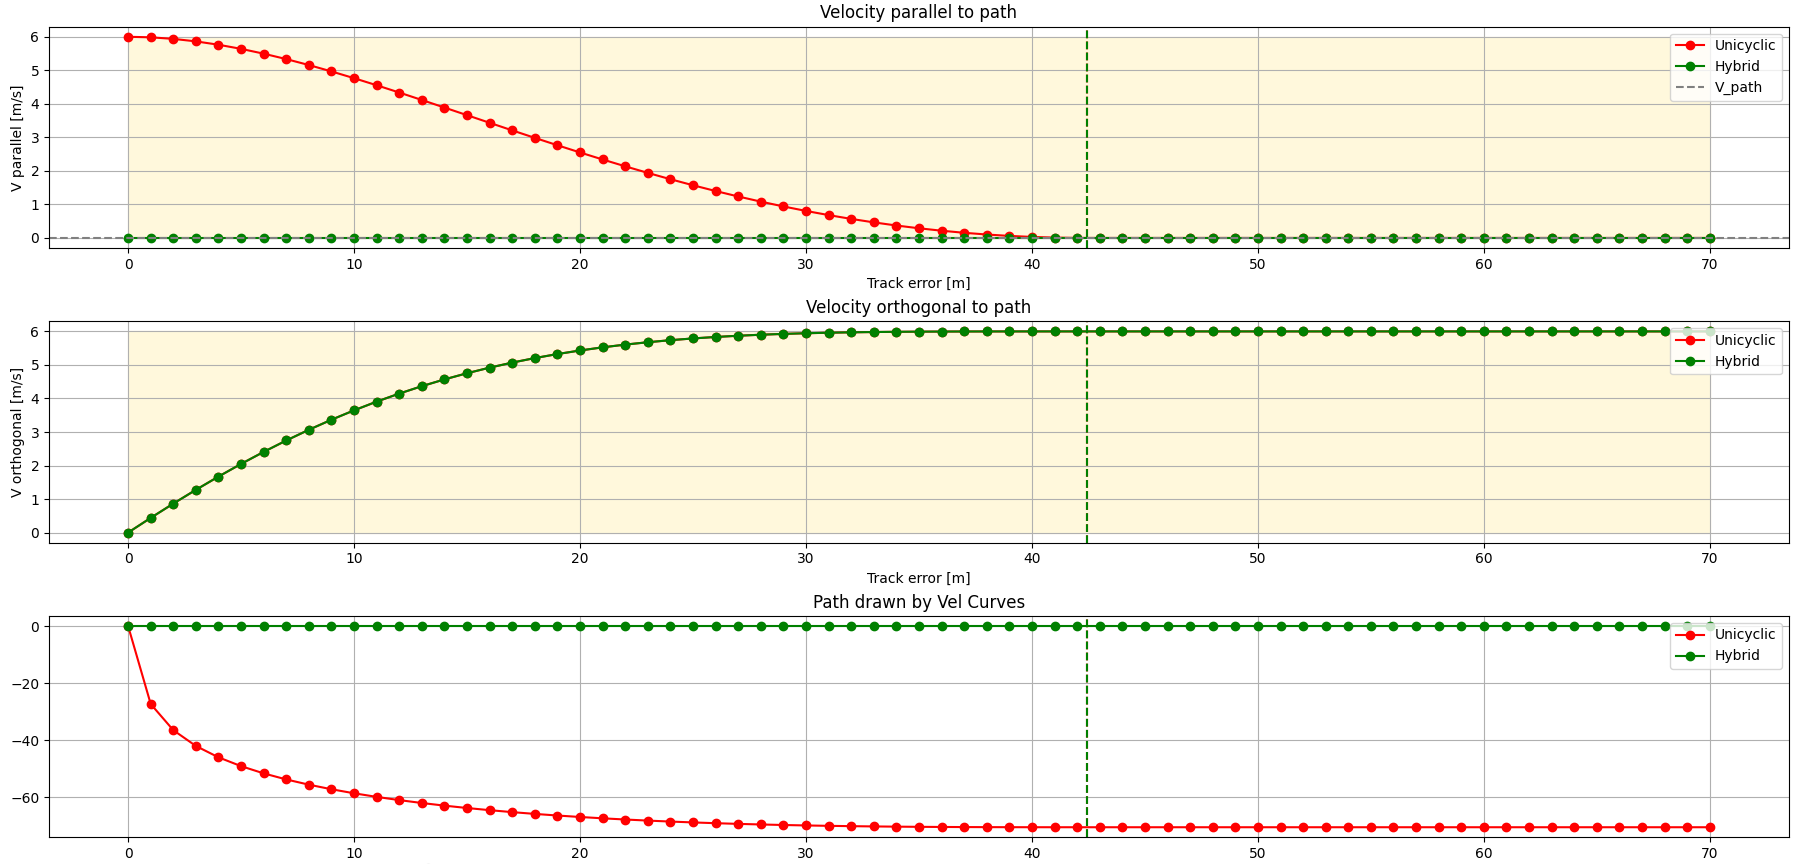
\includegraphics[width=\textwidth]{V_path_0_curve}
\caption{Velocity Curves with zero $V_{path}$}
\end{figure}

\subsection{High Speed On Path}

\includegraphics[width=0.7\textwidth]{VPath_High}

For a high speed on path case, hybrid formulation shows a different approach geometry.

\begin{figure}[h]
\centering
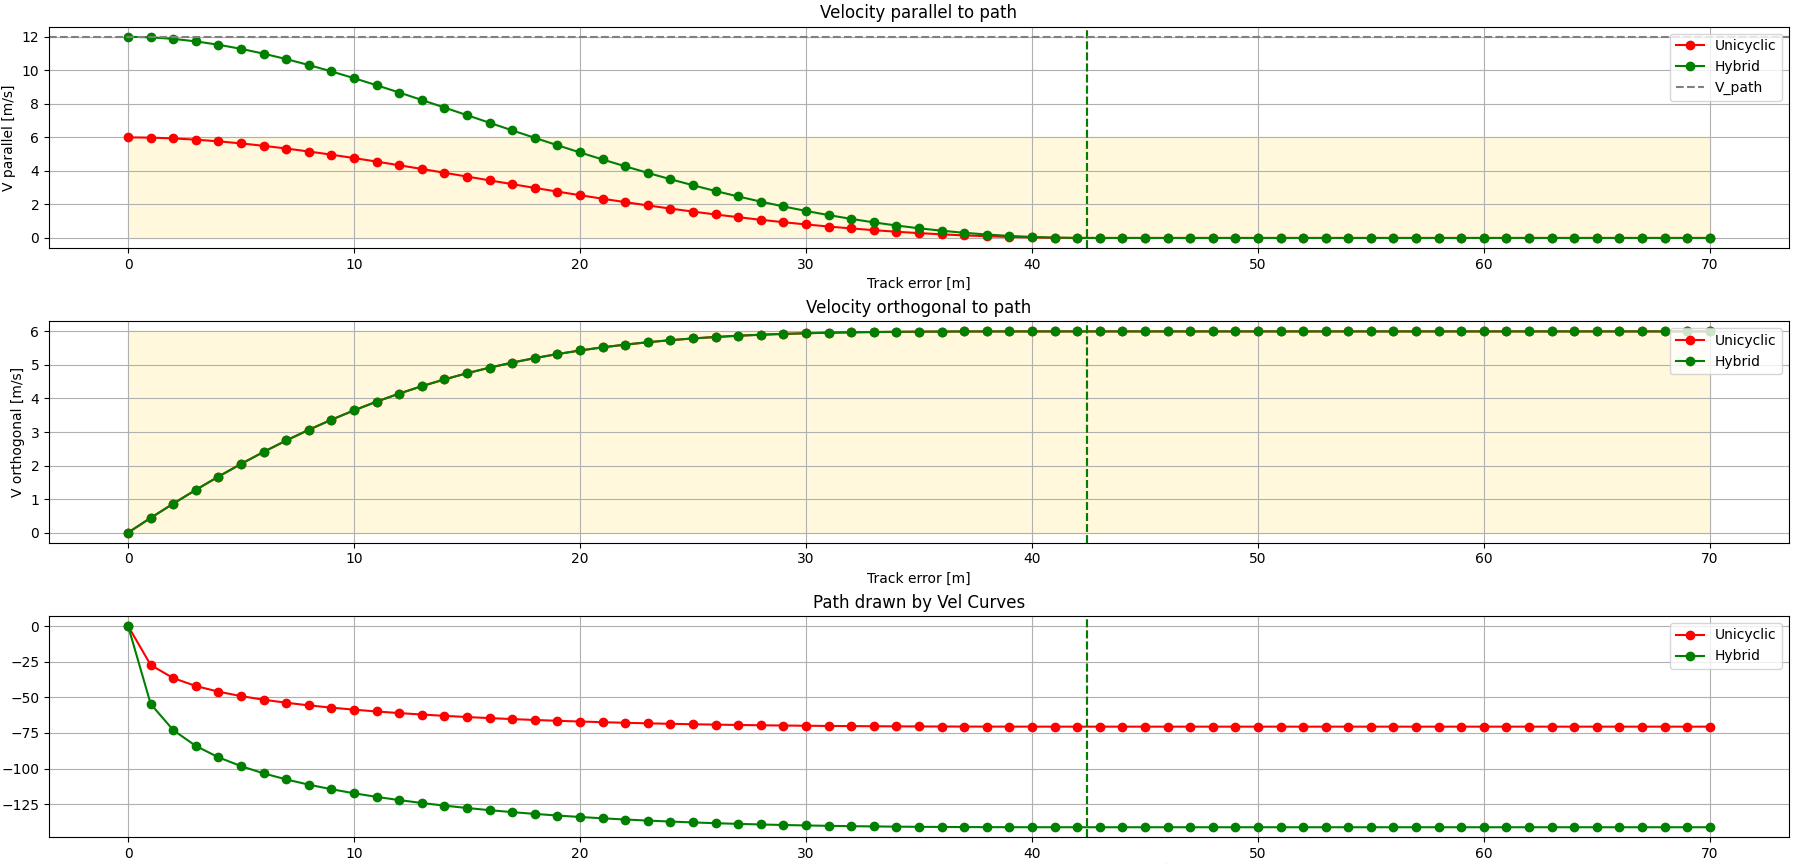
\includegraphics[width=\textwidth]{V_path_12_curve}
\caption{Velocity Curves with high $V_{path}$}
\end{figure}

\section{Acceleration Analysis}

\subsection{Path Orthogonal Acceleration}
The acceleration in the direction orthogonal to the path depends solely on the $V_{ref}^{\perp}(e)$ curve, and assuming vehicle perfectly following the reference velocity vector field, it can be calculated like following:

\begin{equation}
    \begin{split}
    \frac{d}{dt}V_{ref}^{\perp}(e) &= \frac{de}{dt}\frac{d}{de}V_{ref}^{\perp}(e)\\
    &= -V_{ref}^{\perp}(e) \cdot \frac{d}{de}V_{ref}^{\perp}(e)\\
    &= -V_{ref}^{\perp}(e) \cdot \frac{d\overline{e}}{de} \cdot \frac{d}{d\overline{e}}V_{ref}^{\perp}(\overline{e})\\
    &= V_{ref}^{\perp}(e) \cdot \frac{1}{e_b} \cdot V_{approach} \cdot sin(\theta_l(\overline{e})) \cdot \pi (\overline{e} - 1) \\
    &= \frac{V_{approach}^2}{e_b} \cdot \frac{sin(2\theta_l)}{2} \cdot \pi (\overline{e} - 1) \\
    &= \frac{\pi \cdot V_{approach}}{2t_{const}} \cdot sin(\pi (1-\overline{e})) \cdot (\overline{e} - 1)\\
    \end{split}
\label{eq:hybrid_orthogonal_acceleration_derive}
\end{equation}

\begin{figure}[h]
\centering
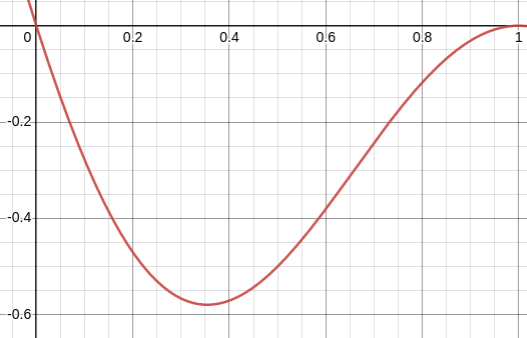
\includegraphics[width=0.6\textwidth]{Orthogonal_acceleration_desmos}
\label{eq:hybrid_orthogonal_acceleration_e_curve}
\end{figure}

Just take the right side of the final equation, this results in the following graph, which deterministically allows us to estimate the acceleration orthogonal to the path when following a track error boundary \autoref{eq:hybrid_track_error_boundary} and look ahead angle \autoref{eq:hybrid_quadratic_laa_curve} as multiplication of the $\frac{\pi \cdot V_{approach}}{2t_{const}}$ term and the graph.\\

And since by numerical analysis, the maximum negative acceleration occurs at $0.3542 \cdot e_b$, with a value of $-0.5792 \cdot \frac{\pi \cdot V_{approach}}{2t_{const}}$, the maximum magnitude of the orthogonal acceleration is determined as $0.9099 \cdot \frac{V_{approach}}{t_{const}}$.\\

Therefore, by picking a conservative value of $t_{const} = \frac{a_{max}^{mc}}{\sqrt{2} V_{approach}}$, the most aggressive approaching behavior can be chosen, which greatly improves the utilization of multirotor's agility compared to a unicyclic approach as demonstrated in the \autoref{tb:unicyclic_hybrid_a_max_comparison} below. Note, the $t_const$ for Unicyclic formulation was retrieved from the original paper\cite{stastny_flying_2019}, which was adapted for the fixed wing use case (thus, larger $t_{const}$).

\begin{table}[h]
\centering
\begin{tabular}{|c | c | c|}
 \hline
  & Unicyclic & Hybrid \\
 \hline
 $a_{max}^{mc} [m/s^2]$ & 10.0 & 10.0 \\ 
 \hline
$V_{approach / nom} [m/s]$ & 10.0 & 10.0 \\ 
 \hline
 $t_{const} [s]$ & 7.071 & 0.7071 \\ 
 \hline
 $a_{max}^{\perp} [m/s^2]$ & \textbf{0.643} & \textbf{6.434} \\
 \hline
\end{tabular}
\caption{Maximum Acceleration Utilized by Unicyclic vs Hybrid Formulation}
\label{tb:unicyclic_hybrid_a_max_comparison}
\end{table}

\section{Monotonicity Analysis}
Since the Velocity setpoint of the Hybrid Formulation\ref{eq:hybrid_velocity_components} is always a point on an ellipse, it is \textbf{guaranteed to be monotonic} as the look-ahead angle $\theta_l$ varies from 0 to $\frac{\pi}{2}$.

\section{Convergence Time Analysis}
Similarly to the acceleration analysis in \autoref{eq:hybrid_orthogonal_acceleration_derive}, convergence time also depends solely on the parameter $t_{const}$, since the absolute magnitude of the velocity was abstractified in \autoref{eq:hybrid_track_error_boundary}.\\

Therefore, since the hybrid formulation can utilize the acceleration constraint more flexibly (as shown in \autoref{tb:unicyclic_hybrid_a_max_comparison}), convergence time to the path is also always faster using the Hybrid formulation.

\section{Fixed Wing Case}

As shown below, the Hybrid formulation still encompasses the unicyclic formulation as a special case, when the $V_{path} = V_{approach}$, which is designated as $V_{nom}$.

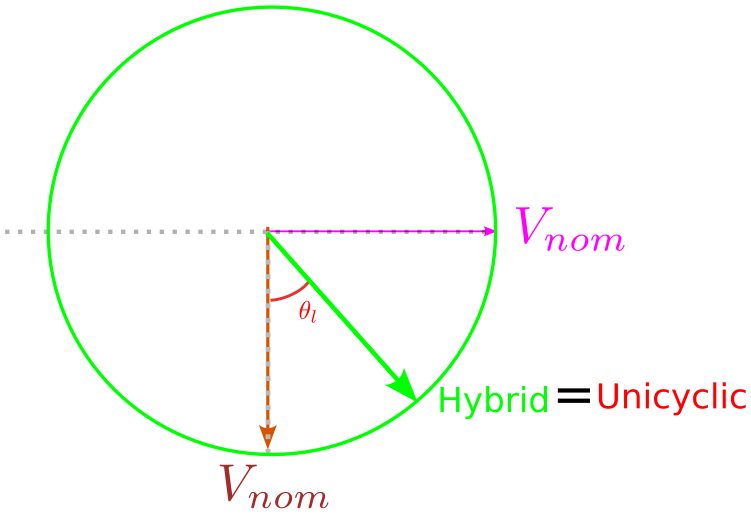
\includegraphics[width=0.7\textwidth]{Hybrid_Supporting_Unicyclic}
% \cleardoublepage

% Conclusion
\chapter{Conclusion}
\label{ch:conclusion}

\begin{figure}[h]
\centering
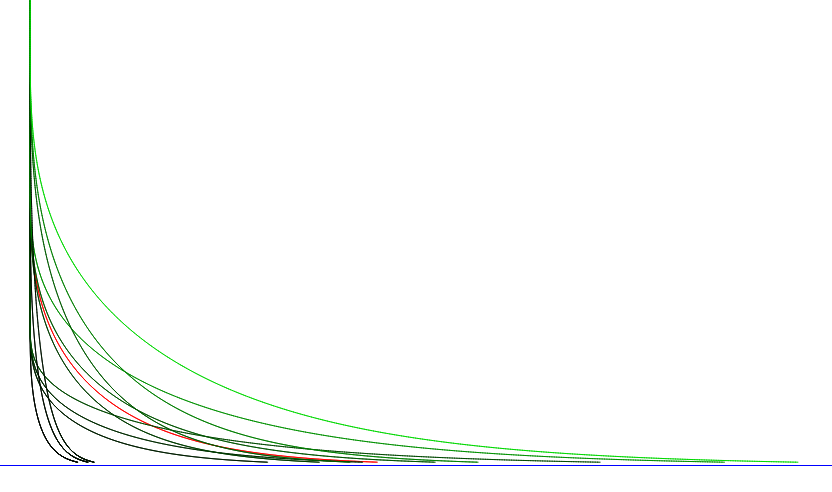
\includegraphics[width=0.7\textwidth]{fun_different_hybrid_path_curves}
\caption{Artwork of different path drawn via Hybrid formulation}
\end{figure}

This thesis successfully demonstrated that unified guidance considering both Multirotor and Fixed Wing use cases for a Hybrid VTOL can be formulated. The Hybrid formulation\ref{eq:hybrid_velocity_components}, was designed to satisfy all the constraints\ref{ch:problem_definition} and hence is a better solution for the use in Hybrid VTOLs.\\

Furthermore, more analysis was given in \autoref{sec:evaluation}, where the superiority of the Hybrid formulation over original Unicyclic method was shown. This is in most part, thanks to the adjustability of the $t_{const}$ appropriately by predicting the acceleration that will occur when following a path beforehand.\\

Note, however that in order to utilize this fully, the real-time adaptation of the $t_{const}$ should be done carefully, to not violate acceleration constraints of different modes of operation.

\section{Future Work}

\subsection{Real Flight Testing}
Unfortunately, the proposed methods were never tested on a real test flight. Implementation of this algorithm on open-source flight control software such as PX4 Autopilot\cite{noauthor_px4_2023} would certainly be possible in the future.

\subsection{Acceleration Limit in Body Frame}
One of the biggest reason why the Maximum Acceleration Method

\subsection{Wind}
Since the acceleration constraint of a Fixed Wing is tied to it's yaw angle, which in turn is tied to the wind vector, it wasn't trivial to come up with a generic solution that would cover all the different wind cases in terms of the acceleration required by the Vector Field.

Therefore, it would be nice to incorporate wind more thoroughly in the guidance algorithm in the future for both Multirotor and Fixed Wing cases to create an actually optimal path following commands, and not just the ground velocity vector field.

\subsection{Low Level Control}
This thesis assumed that the low level controller would be capable of actuating the vehicle to track it's desired ground velocity. However, without the acceleration feed forward command directly computed from the spatial derivative of the Vector Field it would of course be challenging for the low level controller to tightly track the desired velocity.

Therefore, like done in the original unicyclic formulation, it is desirable to passthrough an actual acceleration command in body frame.
% \cleardoublepage

%%%%%%%%%%%%%%%%%%%%%%%%%%%%%%%%%%%%%%%%%%%%%%%%%%%%%%%%%%%%%%%%%%%%%%%%%%%%%%%
% Bibliography
%%%%%%%%%%%%%%%%%%%%%%%%%%%%%%%%%%%%%%%%%%%%%%%%%%%%%%%%%%%%%%%%%%%%%%%%%%%%%%%
\bibliographystyle{bibliography/IEEEtranN}
\bibliography{bibliography/references.bib}
% \printbibliography
\addcontentsline{toc}{chapter}{Bibliography}

%%%%%%%%%%%%%%%%%%%%%%%%%%%%%%%%%%%%%%%%%%%%%%%%%%%%%%%%%%%%%%%%%%%%%%%%%%%%%%%
% Appendix
%%%%%%%%%%%%%%%%%%%%%%%%%%%%%%%%%%%%%%%%%%%%%%%%%%%%%%%%%%%%%%%%%%%%%%%%%%%%%%%
\appendix
\chapter{Maximum Acceleration Limited Path Following Method}
\label{ch:appendix_max_accel}

This is a relaxed maximum acceleration (in path parallel, and orthogonal directions) calculation-based vector field, where we assume that a vehicle approaching at $V_{approach}$ accelerates at the highest possible acceleration to achieve $V_{path}$ while converging to the path.

%%%%%%%%%%%%%%%%%%%%%%%%%%%%%%%%%%%%%%%%%%%5
% ORTHOGONAL VELOCITY
\section{Defining orthogonal velocity curve}

The 'orthogonal' velocity is what actually ties the 'time' - 'track error' relationship ($e(t)$) since the cross track error is only affected by the orthogonal velocity. Theoretically, 'parallel' velocity can have an infinite number of plausible $e(t)$ curves.\newline

Let's take a close look at a typical orthogonal velocity curve in \autoref{fig:v_orth_curve}.

\begin{figure}[h]
\centering
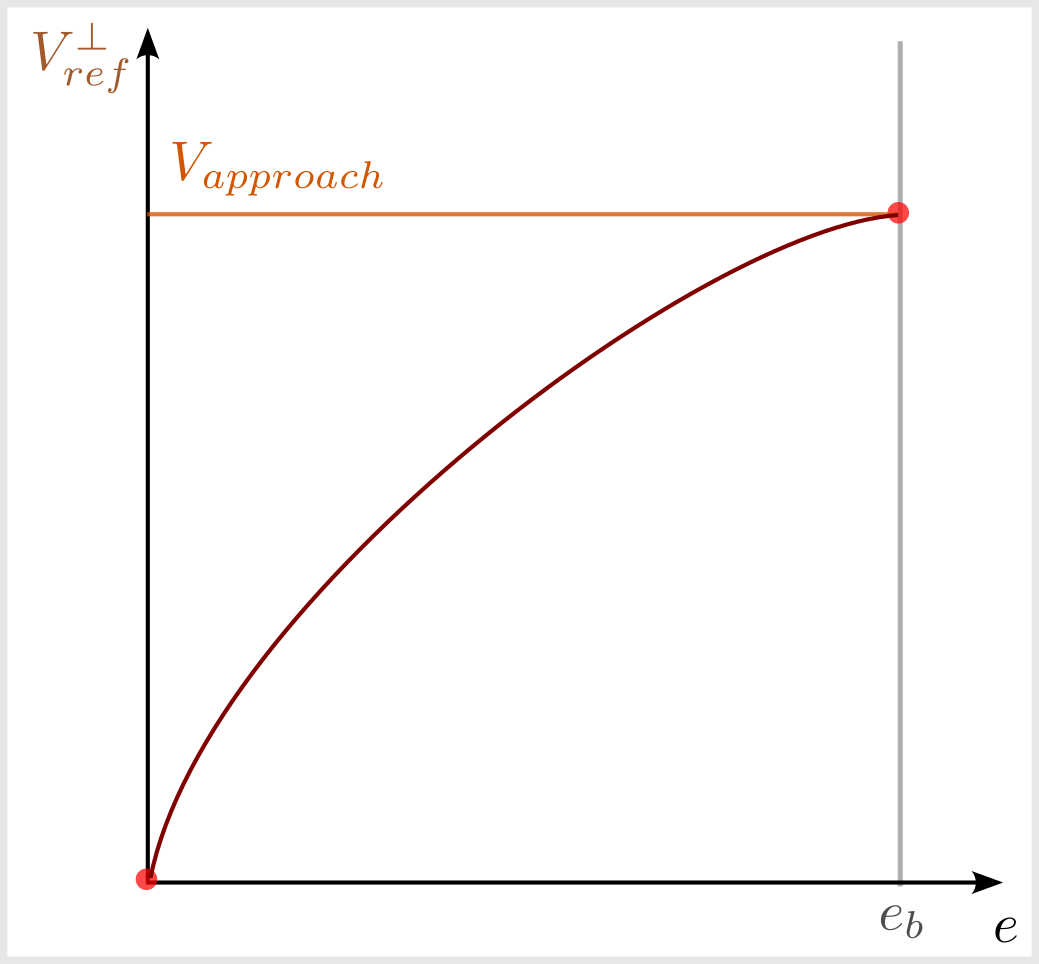
\includegraphics[width=0.5\textwidth]{V_orth_curve_v3.png}
\caption{\label{fig:v_orth_curve}Orthogonal Velocity Curve}
\end{figure}

Here, we define $V_{ref}^{\perp}(e)$, which represents the relationship between orthogonal velocity and cross-track error, as shown in \autoref{fig:v_orth_curve}.

\subsection{Constraints of $V_{ref}^{\perp}$}
To satisfy the entry and on-path conditions, it is clear that the orthogonal velocity curve has a constraint of:

\begin{equation}
%\[
V_{ref}^{\perp}(e)=\begin{cases}
    V_{approach}& \text{if $e = e_b$}\\
    0& \text{if $e = 0$}
\end{cases}
\label{eq:v_orth_constraints}
%\]
\end{equation}

Meaning that at the track error boundary,  approaching velocity must be respected and on path orthogonal velocity must be 0 (to follow the path).\newline

%%%%%%%%%% ACCEL LIMIT
\subsection{Acceleration limited orthogonal velocity profile}

\subsubsection{Derivations of orthogonal velocity curve}
Here is a more in-depth constraint formulation using derivation:

\begin{equation}
    \begin{split}
    \frac{d}{dt}V_{ref}^{\perp}(e) = \frac{de}{dt}\frac{d}{de}V_{ref}^{\perp}(e)\\
    = -V_{ref}^{\perp}(e) * \frac{d}{de}V_{ref}^{\perp}(e)
    \end{split}
\end{equation}

\begin{equation}
\begin{split}
    \text{Therefore, if } &\frac{d}{dt}V_{ref}^{\perp}(e) \geq -a^{\perp}_{max}\\
    &\frac{d}{de}V_{ref}^{\perp}(e) \leq \frac{a^{\perp}_{max}}{V_{ref}^{\perp}}
    \label{eq:accel_limit_orth_vel_deriv}
\end{split}
\end{equation}

This places an upper limit to the derivative of the $V_{ref}^{\perp}(e)$ curve.

\subsubsection{Simple maximum acceleration orthogonal velocity curve}
Using the constraint \autoref{eq:v_orth_constraints}, the 'maximum' acceleration (deceleration) profile of approaching the path can be defined like following:

\begin{equation}
    \text{With orthogonal acceleration limit: } a^{\perp}_{max}
\end{equation}

\begin{equation}
    S^{\perp}_{max-acc} = \{V_{ref}^{\perp}(e) | \ddot{e} = -a^{\perp}_{max}\}
\end{equation}

Where the $S^{\perp}_{max-acc}$ defines the most aggressive curve that is feasible (with a hard deceleration of $-a^{\perp}_{max}$ once the track error enters the track error boundary.\newline

This curve is in fact easily deducible using a constant acceleration equation on a 1-dimensional axis:

\begin{align}
    \text{With } e_b = \frac{V_{approach}^{2}}{2a^{\perp}_{max}}\\
    S^{\perp}_{max-acc}(e)=\begin{cases}
        \sqrt{2a^{\perp}_{max}} * \sqrt{e}& \text{if $e < e_b$}\\
        V_{approach}& \text{if $e \geq e_b$}
    \end{cases}
    \label{eq:s_orth_max_acc}
\end{align}

Particularly, we define the $e_b$ in this case as $e^{min}_{approach}$, which defines the \textbf{minimum required track error to bring $V_{approach}$ to 0 using maximum orthogonal acceleration}.

\begin{equation}
    e^{min}_{approach} = \frac{V_{approach}^{2}}{2a^{\perp}_{max}}
\end{equation}

\begin{figure}[h]
\centering
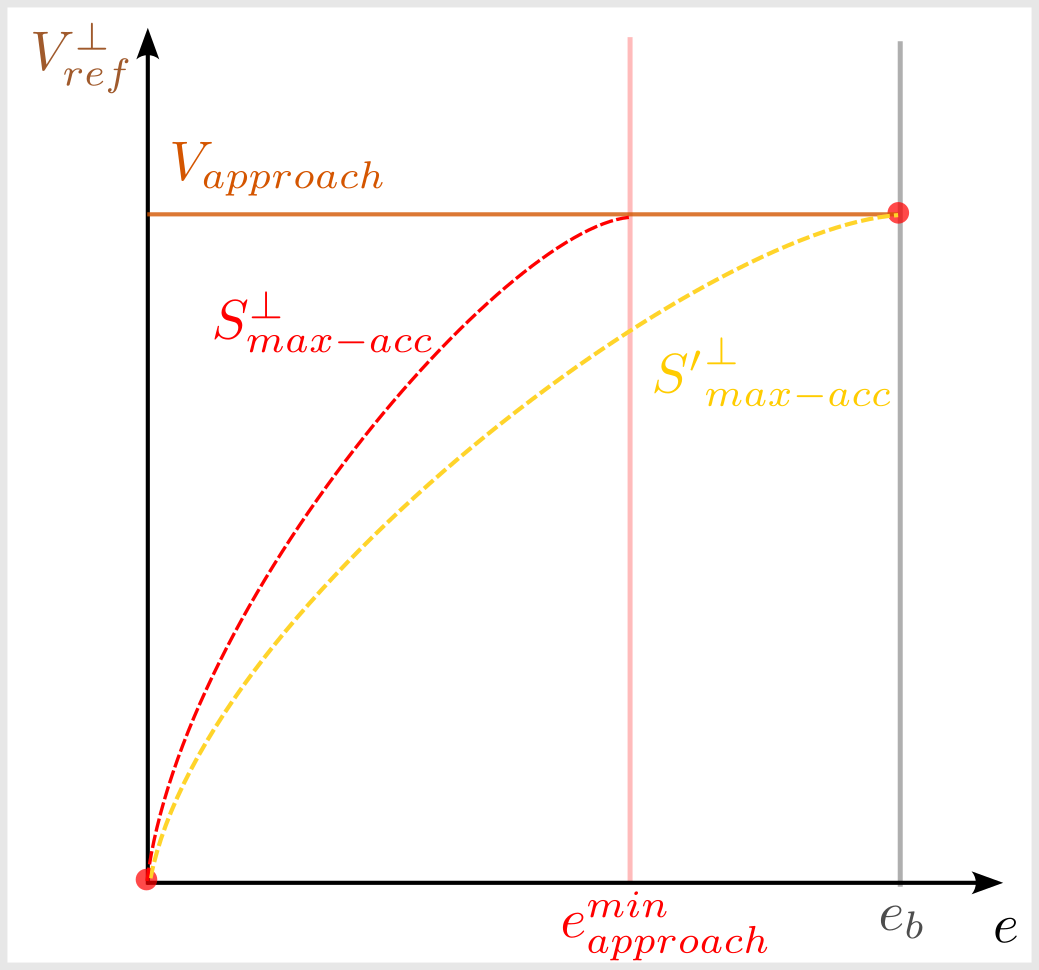
\includegraphics[width=0.5\textwidth]{S_orth_max_acc_v2.png}
\caption{\label{fig:s_orth_max_acc}Maximum orthogonal acceleration curve}
\end{figure}

Note here that $e^{min}_{approach}$ varies by acceleration limit and approach speed. And if we have a constant $e_b$ that we must satisfy (as drawn in \autoref{fig:s_orth_max_acc}), it is simply physically impossible to brake in time without overshooting the path if $e_b$ is smaller than $e^{min}_{approach}$. Therefore, another constraint applies:

\begin{equation}
    e_b \geq e^{min}_{approach}
    \label{eq:e_min_approach_e_b_constraint}
\end{equation}

And as long as the \autoref{eq:e_min_approach_e_b_constraint} and \autoref{eq:accel_limit_orth_vel_deriv} satisfies, \textit{any} curve can be a feasible curve that doesn't exceed maximum orthogonal acceleration limit.

%%%%%%%%%%%% RELAXED MAX ACCEL ORTH VEL
\subsubsection{Relaxed maximum acceleration orthogonal velocity curve}
As noted in the previous section, as long as the \autoref{eq:e_min_approach_e_b_constraint} satisfies, the velocity curve can be drawn. However, how do we actually accommodate the specified $e_b$ into the velocity curve?\newline

To provide a simple solution, a 'relaxed' orthogonal velocity curve  ${S'}^{\perp}_{max-acc}$ can be formulated like the following:

\begin{equation}
\begin{split}
    {S'}^{\perp}_{max-acc}(e) &= {S}^{\perp}_{max-acc}(\frac{e^{min}_{approach}}{e_b} * e)\\
    &=\begin{cases}
        \sqrt{\frac{2a^{\perp}_{max}e^{min}_{approach}}{e_b}} * \sqrt{e}& \text{if $e < e_b$}\\
        V_{approach}& \text{if $e \geq e_b$}
    \end{cases}\\
    &=\begin{cases}
        V_{approach} * \sqrt{\frac{e}{e_b}}& \text{if $e < e_b$}\\
        V_{approach}& \text{if $e \geq e_b$}
    \end{cases}
    \label{eq:relaxed_max_acc_orth_vel_curve}
\end{split}
\end{equation}

Which is basically a \textit{stretched} form of ${S}^{\perp}_{max-acc}$ to match $e^{min}_{approach}$ to specified $e_b$. This satisfies the acceleration derivative constraint (\autoref{eq:accel_limit_orth_vel_deriv}), because the derivative will always be below the upper limit when stretched across the track error axis. This is also illustrated in \autoref{fig:s_orth_max_acc}.\newline

Note that not \textit{every} curve between ${S}^{\perp}_{max-acc}$ and ${S'}^{\perp}_{max-acc}$ is a feasible curve. Because the derivative can go over the upper limit in local sections. Introducing the relaxed maximum acceleration orthogonal velocity curve was in fact motivated by the fact that there are infinite solutions, to provide a simple feasible solution.

%%%%%%%%%%%%%%%%%%%%%%%%%%%%%
% PARALLEL VEL
\section{Parallel Velocity Curve}
Now that we have a theoretical maximum acceleration constrained $V_{ref}^{\perp}(e)$ curve, the parallel Velocity curve can be defined.

% Need to be 400+ dpi to be smooth!
\begin{figure}[h]
\centering
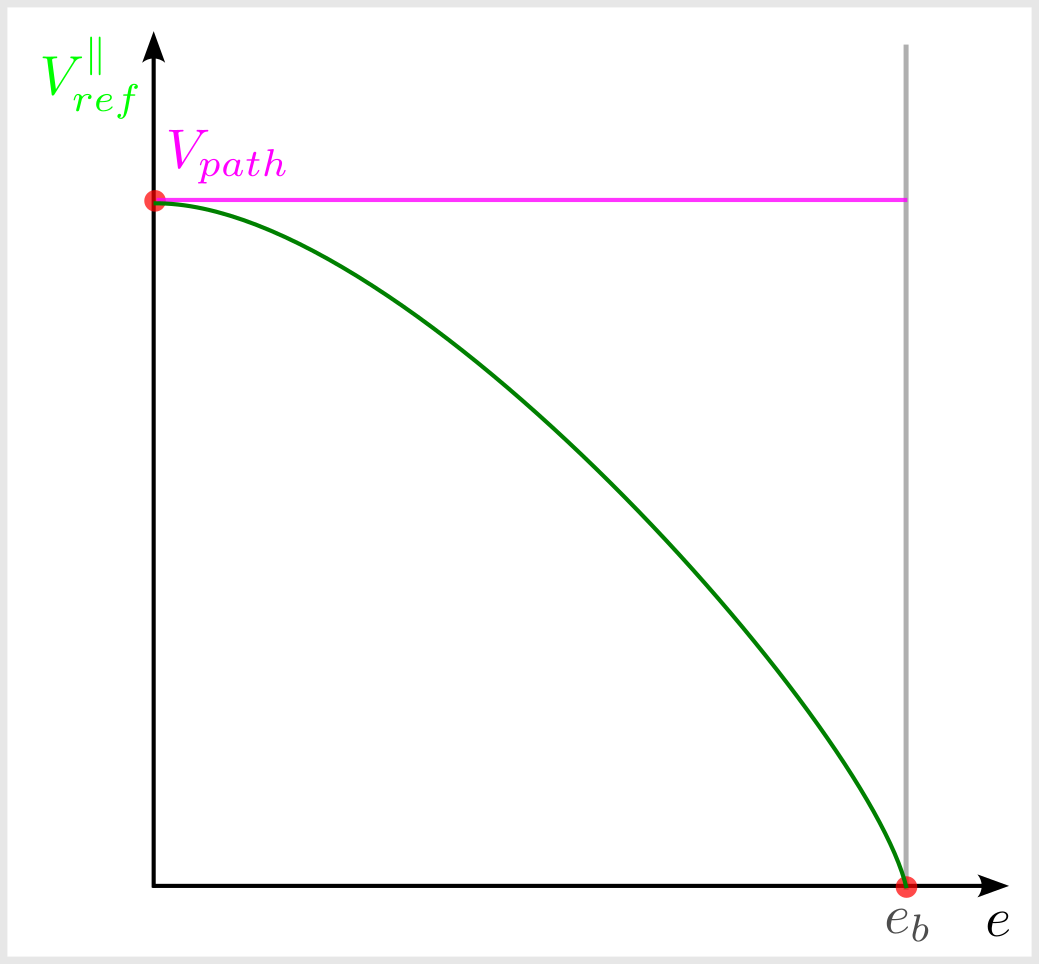
\includegraphics[width=0.5\textwidth]{V_parallel_curve_v3.png}
\caption{\label{fig:v_parallel_curve}Parallel Velocity Curve}
\end{figure}

\subsection{Constraints of $V_{ref}^{\parallel}(e)$}
To respect the boundary/on-path conditions, it is clear that the parallel velocity curve has a constraint of:

\begin{equation}
V_{ref}^{\parallel}(e)=\begin{cases}
    0& \text{if $e = e_b$}\\
    V_{path}& \text{if $e = 0$}
\end{cases}
\label{eq:v_parallel_constraints}
\end{equation}

\subsection{Acceleration limited parallel velocity profile}
First constraint that applies to $V_{ref}^{\parallel}(e)$ is it's acceleration along the direction parallel to the path. This can be derived easily, but with a dependency to orthogonal velocity curve.

\begin{equation}
    \text{With parallel acceleration limit: } a^{\parallel}_{max}
\end{equation}

\begin{equation}
    S^{\parallel}_{max-acc} = \{V_{ref}^{\parallel}(e) | \ddot{V}_{ref}^{\parallel}(e) = a^{\parallel}_{max}\}
\end{equation}

If we apply the derivation:

\begin{equation}
    \begin{split}
    \frac{d}{dt}V_{ref}^{\parallel}(e) = \frac{de}{dt}\frac{d}{de}V_{ref}^{\parallel}(e)\\
    = -V_{ref}^{\perp}(e) * \frac{d}{de}V_{ref}^{\parallel}(e)
    \end{split}
\end{equation}

% https://tex.stackexchange.com/questions/384299/splitting-lines-for-long-equations
\begin{equation}
\begin{split}
    \text{Therefore, if } &\frac{d}{dt}V_{ref}^{\parallel}(e) \leq a^{\parallel}_{max},\\
    &\frac{d}{de}V_{ref}^{\parallel}(e) \geq -\frac{a^{\parallel}_{max}}{V_{ref}^{\perp}(e)}
\end{split}
\end{equation}

This puts a lower bound on the derivative of $V_{ref}^{\parallel}(e)$, defining how aggressively the parallel velocity can decrease along cross-track error ($e$).\newline

%%%%%%%%%% Paralle velocity constraint with relaxed orth vel curve
\subsubsection{Maximum acceleration parallel velocity with relaxed max orthogonal velocity curve}
It should be noted that by substituting the relaxed maximum acceleration orthogonal velocity curve (\autoref{eq:relaxed_max_acc_orth_vel_curve}) to $V^{\perp}_{ref}(e)$, the constraint becomes:

\begin{equation}
\begin{split}
    \frac{d}{de}V_{ref}^{\parallel}(e) &\geq -\frac{a^{\parallel}_{max}}{{S'}^{\perp}_{max-acc}(e)}\\
    &=\begin{cases}
        -\frac{a^{\parallel}_{max}}{V_{approach}} * \sqrt{\frac{e_b}{e}}& \text{if $e < e_b$}\\
        -\frac{a^{\parallel}_{max}}{V_{approach}}& \text{if $e \geq e_b$}
    \end{cases}
\end{split}
\end{equation}

Also, considering boundary constraints in \autoref{eq:v_parallel_constraints}, it should be noted that another constraint must be satisfied between $V_{path}$ and $e_b$, since if the $V_{path}$ is too large, it would be impossible to reach the desired speed on path with a given $e_b$ distance to track. Therefore, we must compute the 'maximum' $V_{path}$ achievable with a given constraints:

\begin{equation}
    \begin{split}
        V_{path}^{max} |_{S'^{\perp}_{max-acc}} &= S^{\parallel}_{max-acc}(e=0)\\
        &= \int^{0}_{e_b}{-\frac{a^{\parallel}_{max}}{V_{approach}}\sqrt{\frac{e_b}{e}}} de\\
        &= -\frac{a^{\parallel}_{max}\sqrt{e_b}}{V_{approach}} * [2\sqrt{e}]^{0}_{e_b}\\
        &= \frac{2a^{\parallel}_{max}e_b}{V_{approach}}
    \end{split}
    \label{eq:max_path_speed_with_relaxed_orthog_speed_max_acc}
\end{equation}

Therefore, if $V_{path}$ is greater than the calculated $V_{path}^{max} |_{S'^{\perp}_{max-acc}}$, the parallel velocity curve is simply infeasible with the parallel acceleration constraints. And it is in fact possible to calculate the minimum track error boundary required to achieve the speed on path.

\begin{equation}
\begin{split}
    \text{Since } V_{path} &= \int_{e^{min}_{path}}^{0}-\frac{a^{\parallel}_{max}}{V_{approach}}\sqrt{\frac{e_b}{e}}de,\\
    &= -\frac{a^{\parallel}_{max}\sqrt{e_b}}{V_{approach}} * [2\sqrt{e}]^{0}_{e^{min}_{path}},\\
    \text{Therefore, } e^{min}_{path}|_{S'^{\perp}_{max-acc}} &= [\frac{V_{path}V_{approach}}{2a^{\parallel}_{max}}]^2*\frac{1}{e_b}
\end{split}
\end{equation}

Which defines the minimum track error point where acceleration in parallel velocity should be applied, with the given relaxed maximum acceleration orthogonal velocity curve $S'^{\perp}_{max-acc}$.\newline

Using this, we can formulate the maximum acceleration parallel velocity curve dependent on relaxed orthogonal velocity:

\begin{align}
    S^{\parallel}_{max-acc}(e)=\begin{cases}
        V_{path} - \frac{2a^{\parallel}_{max}\sqrt{e_b}}{V_{approach}} * \sqrt{e}& \text{if $e < e^{min}_{path}|_{S'^{\perp}_{max-acc}}$}\\
        0& \text{if $e \geq e^{min}_{path}|_{S'^{\perp}_{max-acc}}$}
    \end{cases}
    \label{eq:s_orth_max_acc}
\end{align}

\begin{figure}[h]
\centering
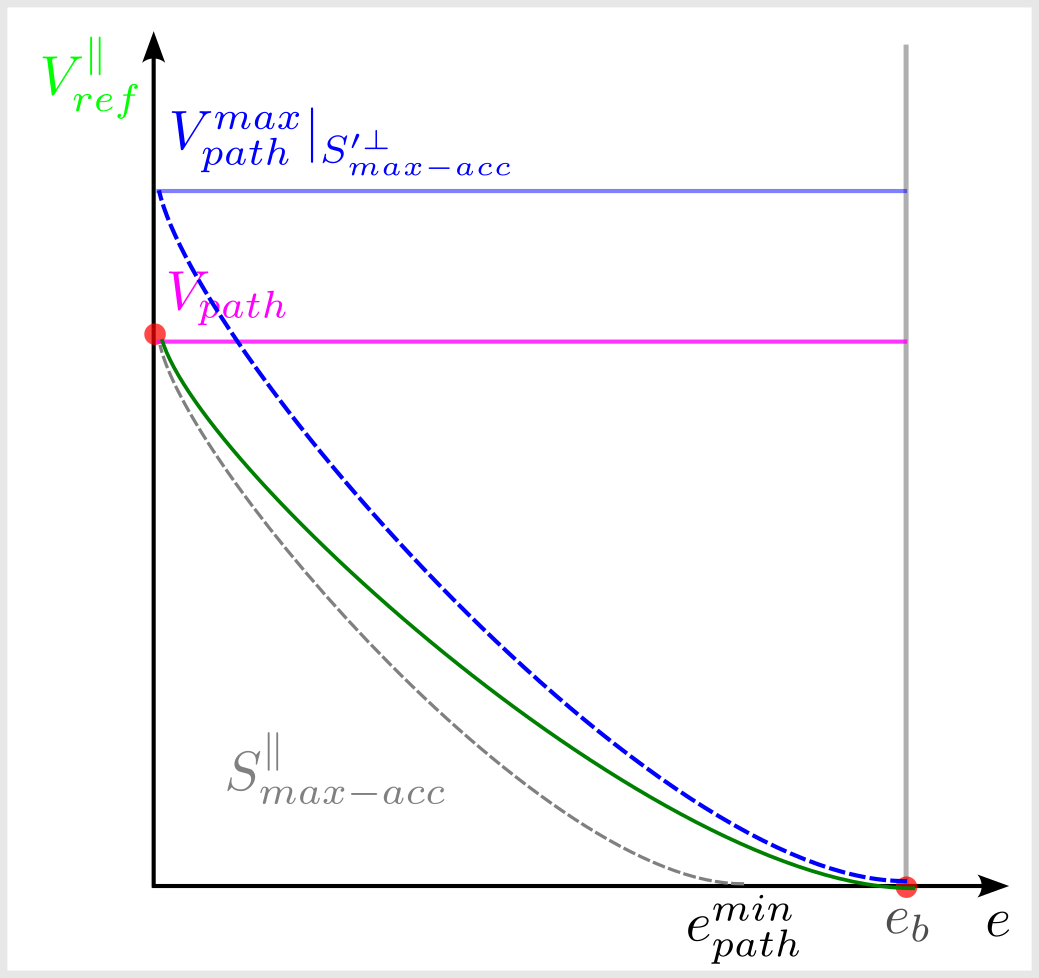
\includegraphics[width=0.5\textwidth]{S_parallel_max_acc_v2.png}
\caption{\label{fig:acc_limited_parallel_vel}Acceleration limited parallel velocity curve}
\end{figure}

\subsubsection{Relaxed parallel velocity curve with relaxed orthogonal velocity curve}
Similarly to orthogonal velocity curve's case, the $e^{min}_{path}|_{S'^{\perp}_{max-acc}}$ doesn't equal to $e_b$ all the time. Therefore, we introduce another relaxed parallel velocity curve that satisfies the acceleration limits:

\begin{equation}
\begin{split}
    {S'}^{\parallel}_{max-acc}(e) &= {S}^{\parallel}_{max-acc}(\frac{e^{min}_{path}|_{S'^{\perp}_{max-acc}}}{e_b} * e)\\
    &=\begin{cases}
        V_{path} - \frac{2a^{\parallel}_{max}\sqrt{e_b}}{V_{approach}} * \sqrt{\frac{e^{min}_{path}|_{S'^{\perp}_{max-acc}}}{e_b} * e}& \text{if $e < e_b$}\\
        0& \text{if $e \geq e_b$}
    \end{cases}\\
    &=\begin{cases}
        V_{path} * (1 - \sqrt{\frac{e}{e_b}})& \text{if $e < e_b$}\\
        0& \text{if $e \geq e_b$}
    \end{cases}
    \label{eq:relaxed_max_acc_parallel_vel_curve}
\end{split}
\end{equation}

This is a very similar form to \autoref{eq:relaxed_max_acc_orth_vel_curve}, as the velocities get ramped in/out proportional to $\sqrt{\frac{e}{e_b}}$.

\subsection{Velocity norm Monotonicity}
Another constraint is to make sure vehicle doesn't brake and accelerate, but rather have a constantly decreasing velocity norm profile when approaching path. This is desired since it gives a smooth speed curve, which can have higher efficiency (to be clarified), and more intuitive path following behavior.

\begin{equation}
    \dot{|V_{ref}|} \leq 0
\end{equation}

Since derivative of the velocity curves against track error ($e$), when multiplied by $-V^{\perp}_{ref}$ gives the derivative against time, this can be formulated as:

\begin{equation}
    \begin{split}
        \dot{|V_{ref}|} &= \dot{\sqrt{{V_{ref}^{\parallel}}^2 + {V_{ref}^{\perp}}^2}}\\
        &= \frac{1}{|V_{ref}|} * (\dot{V}_{ref}^{\parallel} + \dot{V}_{ref}^{\perp})\\
        &= \frac{-V^{\perp}_{ref}}{|V_{ref}|} * (\frac{{dV}_{ref}^{\parallel}}{de} + \frac{{dV}_{ref}^{\perp}}{de})\\
        \text{Therefore, } &\frac{{dV}_{ref}^{\parallel}}{de} + \frac{{dV}_{ref}^{\perp}}{de} \geq 0
    \end{split}
\end{equation}

\subsubsection{Monotonicity constraint on relaxed curves}
Using \autoref{eq:relaxed_max_acc_orth_vel_curve} and \autoref{eq:relaxed_max_acc_parallel_vel_curve}:

\begin{equation}
\begin{split}
    \frac{{dV}_{ref}^{\parallel}}{de} + \frac{{dV}_{ref}^{\perp}}{de} = \frac{V_{approach}-V_{path}}{\sqrt{e_b}} * \frac{1}{2\sqrt{e}} \geq 0
\end{split}
\end{equation}

This indicates that for our relaxed curves to satisfy monotonically reducing velocity form as it approaches the path, the approach velocity must be bigger than velocity on path.

% \chapter{Irgendwas}\label{sec:irgendwas}

Bla bla \dots
% \cleardoublepage
% \chapter{Datasheets}\label{sec:datasheets}

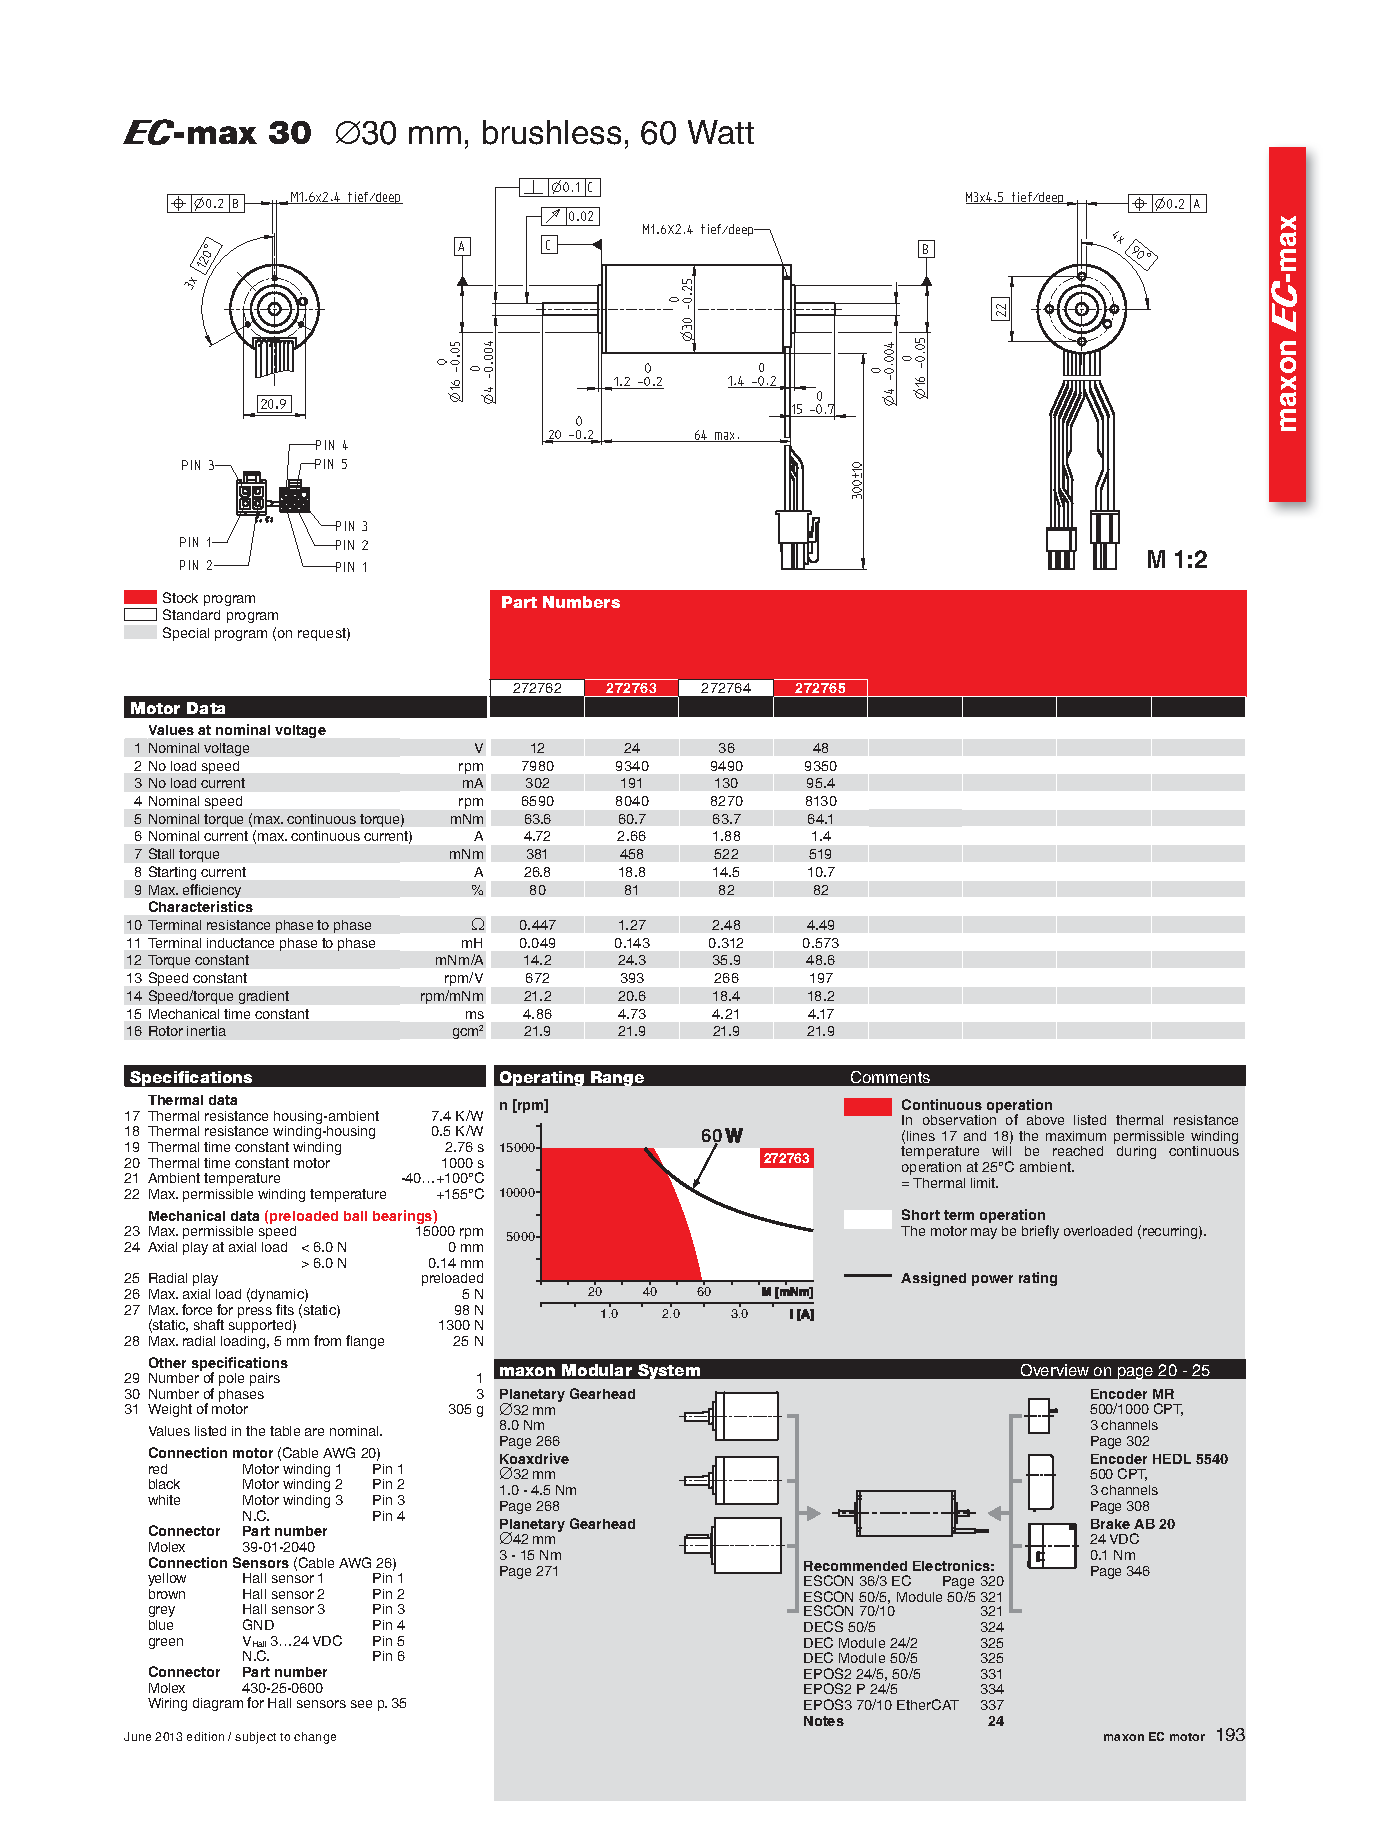
\includepdf[scale=0.75]{images/datasheets.pdf}

\end{document}